\chapter{Genómica y secuenciación}\label{ch:b3:genomics}

El primer genoma completo de un organismo de vida libre, las
\qty{1.8}{Mb} de una bacteria, se publicó en 1995 tras un año de trabajo
de un equipo de cuarenta personas. El genoma humano, \num{3.2} mil
millones de pares de bases, le costó a un consorcio internacional trece
años y unos tres mil millones de dólares, y se declaró terminado en 2003.
Hoy una máquina de sobremesa lee un genoma humano en una noche por unos
pocos centenares de dólares, un hospital secuencia el tumor de un
paciente para elegir un fármaco y un museo extrae y lee el genoma de un
hueso de cuarenta mil años. La tecnología que ha hecho esto posible, la
matemática que convierte millones de \omterm{def:b3:genomics:ngs}{lecturas} cortas en un genoma y lo
que los genomas terminados han enseñado sobre el tamaño, el contenido y
la historia de nuestro ADN son el asunto de este capítulo. El capítulo
siguiente retoma los algoritmos que comparan las secuencias ya obtenidas.

\section{Leer el ADN}

\begin{definition}[Secuenciación por terminación de cadena]\label{def:b3:genomics:sanger}
\index{secuenciación de Sanger}\index{didesoxinucleótido}\index{terminación de cadena}
La \emph{secuenciación de Sanger} copia un molde de hebra sencilla a
partir de un cebador con ADN-polimerasa en presencia de los cuatro
nucleótidos normales y de una pequeña proporción de
\emph{didesoxinucleótidos}, que carecen del hidroxilo 3$'$ y terminan por
tanto la cadena allí donde se incorporan. Cada didesoxinucleótido lleva
un fluoróforo distinto. El producto es una mezcla de fragmentos, uno por
cada posición del molde, y cada uno acaba en una base de identidad
conocida; separados por tamaño en un capilar de gel, pasan por un
detector en orden de longitud, y la secuencia de colores es la secuencia
del molde. Una carrera lee \qtyrange{700}{900}{bp} con una tasa de error
por debajo de $10^{-3}$; sigue siendo el método para verificar una
construcción o un solo gen.
\end{definition}

\begin{proof}[Evidencia]
Sanger, Nicklen y Coulson publicaron el método en 1977 y lo usaron ese
mismo año para leer los \qty{5386}{bp} del fago $\phi$X174 --- el primer
genoma de ADN completo --- y en 1981 los \qty{16569}{bp} de la
mitocondria humana. Fleischmann y colaboradores (1995) leyeron las
\qty{1.83}{Mb} de \emph{Haemophilus influenzae} rompiendo todo el genoma
en fragmentos al azar, secuenciando \num{24000} de ellos y ensamblando
las \omterm{def:b3:genomics:ngs}{lecturas} por ordenador --- la estrategia de \emph{escopetazo del
genoma completo} que todos los proyectos posteriores ampliaron.
\end{proof}

\begin{omfigure}
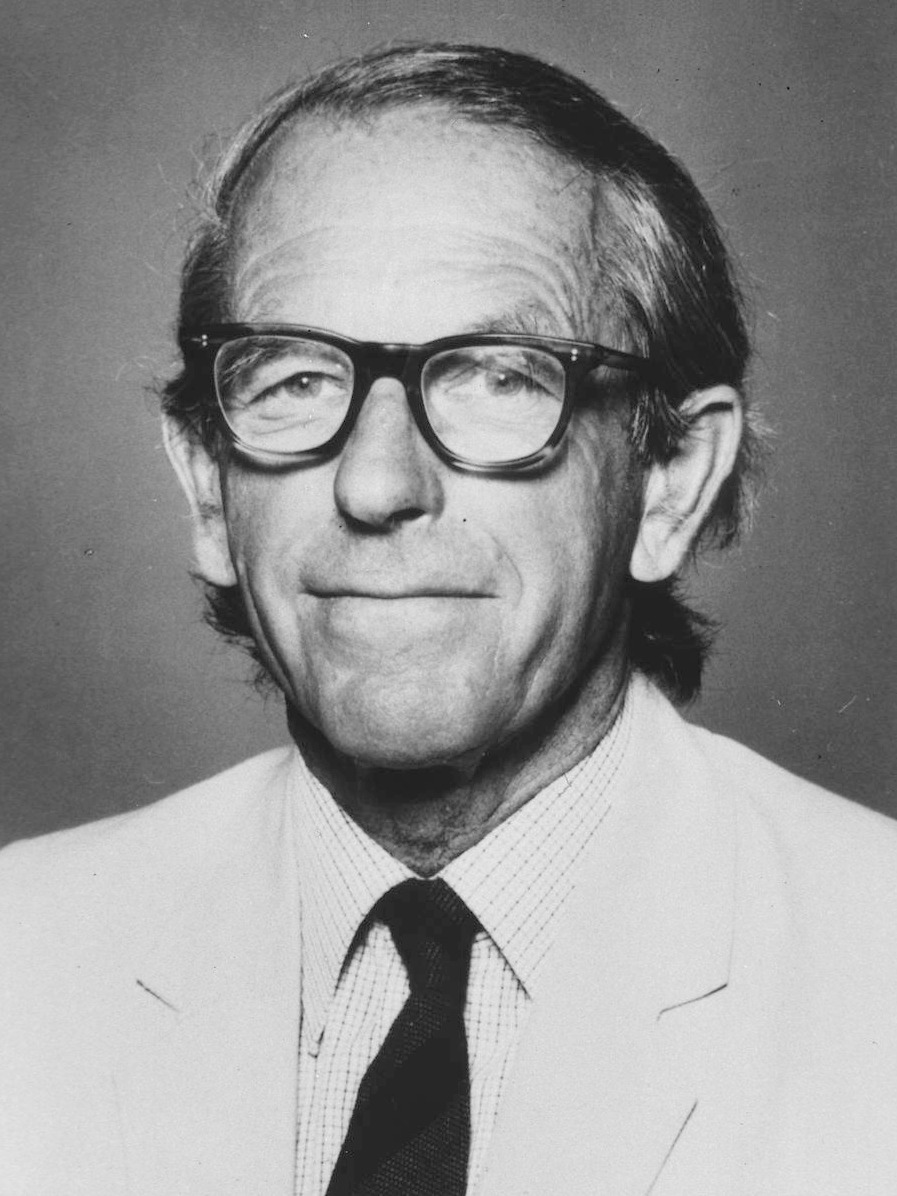
\includegraphics[width=0.30\linewidth]{images/book5/sanger.jpg}\hspace{0.04\linewidth}
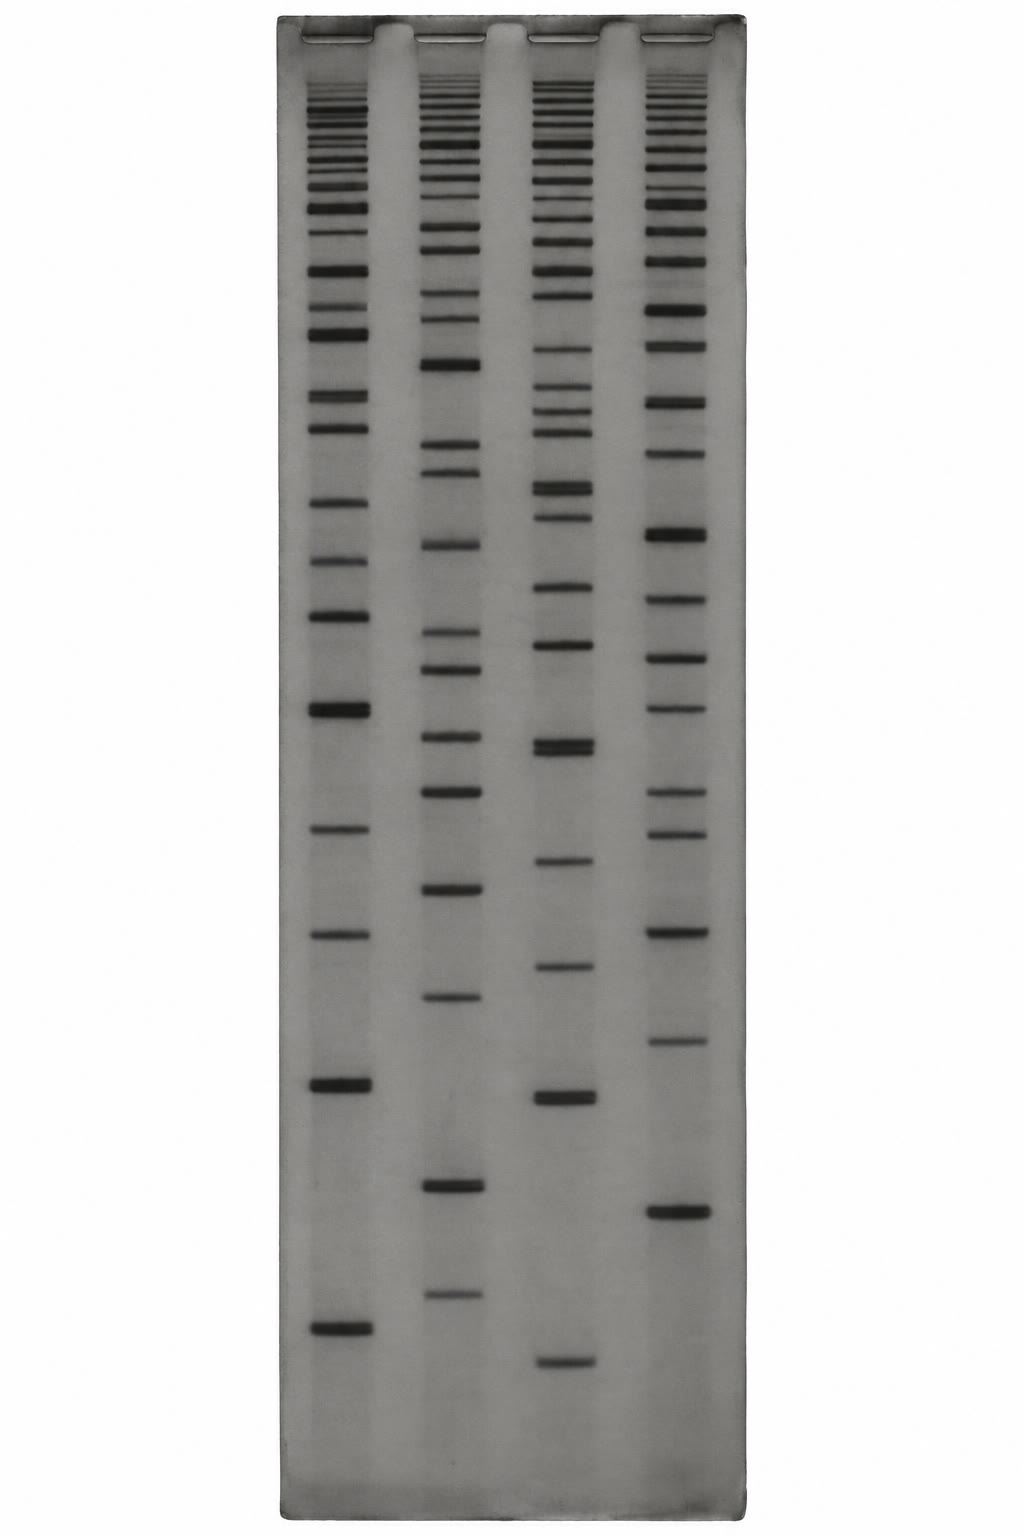
\includegraphics[width=0.30\linewidth]{images/book5/ai/b5-04-sanger-gel.jpg}

{\small Izquierda: Frederick Sanger, que ideó los primeros métodos
prácticos para leer proteínas y ADN y recibió un premio Nobel por cada
uno. Derecha: una autorradiografía de un gel de secuenciación de la era
anterior al capilar, con una calle por base y la secuencia leída de abajo
arriba en la escalera de bandas.}
\end{omfigure}

\begin{omfigure}
\begin{tikzpicture}[every node/.style={font=\scriptsize}, >=stealth]
  % template and primer
  \draw[very thick, omDef] (0,3.0) -- (6,3.0); \node[left] at (-0.1,3.0) {molde 3$'$};
  \node[right] at (6.05,3.0) {5$'$};
  \foreach \x/\b in {0.6/T,1.2/G,1.8/A,2.4/C,3.0/T,3.6/T,4.2/G,4.8/C} \node[above, omDef] at (\x,3.05) {\b};
  \draw[very thick, omProp] (0,2.6) -- (0.3,2.6); \node[left] at (-0.1,2.6) {cebador};
  % terminated products
  \foreach \i/\len/\col/\b in {1/0.6/omDef/A, 2/1.2/omMeth/C, 3/1.8/omThm/T, 4/2.4/omExo/G, 5/3.0/omDef/A, 6/3.6/omDef/A, 7/4.2/omMeth/C, 8/4.8/omExo/G} {
    \draw[very thick, omProp] (0,2.6-0.32*\i) -- (\len-0.15,2.6-0.32*\i);
    \fill[\col] (\len-0.05,2.6-0.32*\i) circle (0.1);
    \node[right, \col] at (\len+0.05,2.6-0.32*\i) {dd\b};
  }
  \node[below, align=center] at (2.4,-0.25) {un producto por cada posición, cada uno terminado\\en una base didesoxi fluorescente};
  % capillary readout
  \draw[->, thick] (6.5,1.3) -- (7.4,1.3) node[midway, above] {tamaño};
  \draw[thick] (7.6,0.0) rectangle (11.6,2.6);
  \foreach \i/\col in {1/omDef, 2/omMeth, 3/omThm, 4/omExo, 5/omDef, 6/omDef, 7/omMeth, 8/omExo} {
    \draw[very thick, \col] (7.6+0.45*\i,0.1) .. controls (7.6+0.45*\i-0.15,0.1) and (7.6+0.45*\i-0.1,1.6) .. (7.6+0.45*\i,1.6) .. controls (7.6+0.45*\i+0.1,1.6) and (7.6+0.45*\i+0.15,0.1) .. (7.6+0.45*\i+0.3,0.1);
  }
  \foreach \i/\b in {1/A, 2/C, 3/T, 4/G, 5/A, 6/A, 7/C, 8/G} \node[above] at (7.6+0.45*\i,1.7) {\b};
  \node[below] at (9.6,-0.05) {más corto $\to$ más largo: la secuencia, leída en color};
\end{tikzpicture}

{\small La secuenciación por \omterm{def:b3:genomics:sanger}{terminación de cadena}. Una base didesoxi
termina la copia en cada posición donde se incorpora; los fragmentos, uno
por longitud, se separan por tamaño y el color de cada base terminal se
lee en orden.}
\end{omfigure}

\begin{definition}[Secuenciación masiva en paralelo]\label{def:b3:genomics:ngs}
\index{secuenciación por síntesis}\index{lectura}\index{secuenciación de lectura larga}\index{nanoporo}
Los instrumentos de segunda generación leen de millones a miles de
millones de fragmentos a la vez. En la \emph{secuenciación por síntesis}
los fragmentos, con adaptadores ligados a sus extremos, se fijan a una
celda de flujo de vidrio y se amplifican in situ en agrupaciones de
moléculas idénticas; las agrupaciones se alargan luego una base por ciclo
con nucleótidos fluorescentes y bloqueados de forma reversible, se
fotografían, se desbloquean y se vuelven a alargar, de modo que cada
ciclo añade una base a la \emph{lectura} de cada agrupación. Las lecturas
son de \qtyrange{100}{300}{bp}, casi siempre desde los dos extremos de un
fragmento (\emph{extremos emparejados}), con una tasa de error de unos
$10^{-3}$ por base, y una carrera rinde hasta $10^{12}$ bases. Los
instrumentos de tercera generación, de \emph{lectura larga}, leen
moléculas sueltas sin amplificación: observando cómo una polimerasa
incorpora nucleótidos fluorescentes en tiempo real, o haciendo pasar el
ADN por un \emph{nanoporo} proteico y registrando la corriente iónica,
que cada secuencia de bases modula a su manera. Las lecturas de
\qtyrange{10}{100}{kb} y más abarcan las repeticiones que las lecturas
cortas no pueden, con una tasa bruta de error mayor que el consenso
reduce.
\end{definition}

\begin{omfigure}
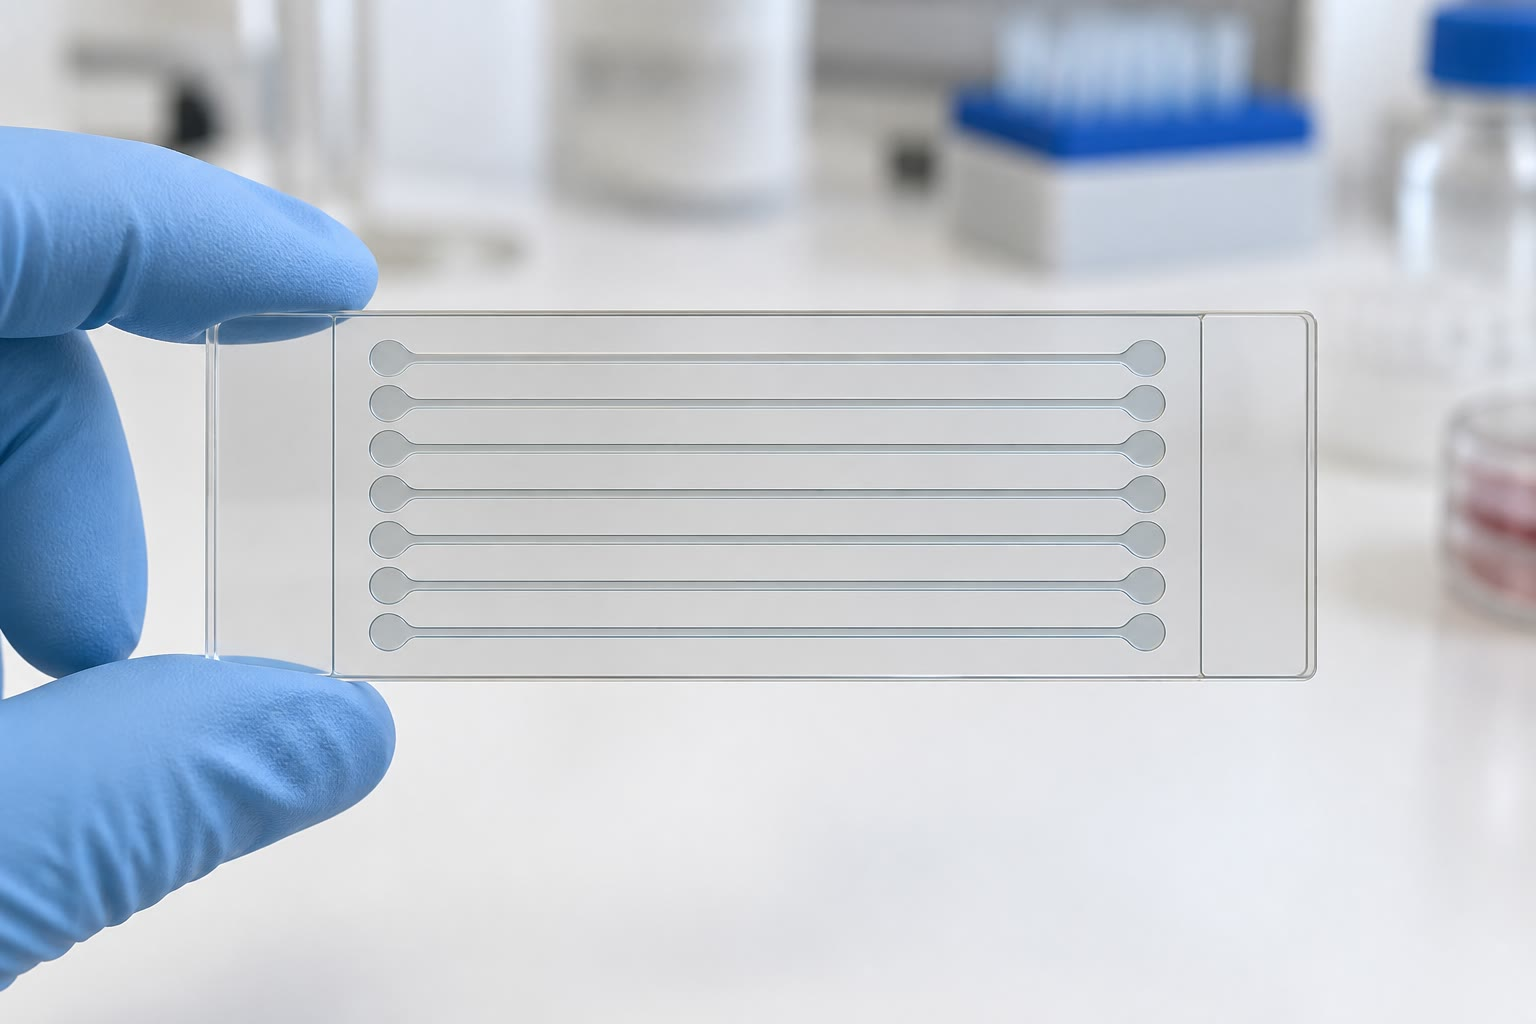
\includegraphics[width=0.46\linewidth]{images/book5/ai/b5-04-flowcell.jpg}\hspace{0.04\linewidth}

\includegraphics[width=0.46\linewidth]{images/book5/ai/b5-04-nanopore.jpg}

{\small Izquierda: una celda de flujo, el portaobjetos de vidrio sobre el
que se hacen crecer y se leen miles de millones de agrupaciones de ADN a
razón de una base por ciclo. Derecha: un secuenciador de \omterm{def:b3:genomics:ngs}{nanoporos} de
bolsillo que lee moléculas sueltas como cambios de una corriente iónica.}
\end{omfigure}

\begin{theorem}[Cobertura y huecos en un proyecto de escopetazo]\label{thm:b3:genomics:lander-waterman}
\index{cobertura}\index{Lander--Waterman}\index{contig}
Tómense $N$ \omterm{def:b3:genomics:ngs}{lecturas} de longitud $L$ en posiciones aleatorias de un
genoma de longitud $G$, y sea $c = NL/G$ la \emph{cobertura}, el número
medio de \omterm{def:b3:genomics:ngs}{lecturas} que cubren una base. El número de \omterm{def:b3:genomics:ngs}{lecturas} que cubre
una base dada sigue entonces una Poisson de media $c$: la fracción del
genoma que queda sin secuenciar es
\[
P(\text{sin cubrir}) = e^{-c},
\]
y si dos \omterm{def:b3:genomics:ngs}{lecturas} se reconocen como solapadas solo cuando comparten al
menos $T$ bases, de modo que $\theta = T/L$, el número esperado de
\emph{contigs} (islas de \omterm{def:b3:genomics:ngs}{lecturas} solapadas) es
\[
\text{contigs} = N\,e^{-c(1-\theta)},
\]
y su longitud media es $L\,\bigl(e^{c(1-\theta)} - 1\bigr)/c + L\theta$,
aproximadamente.
\end{theorem}
\begin{proof}
Los puntos de inicio de las \omterm{def:b3:genomics:ngs}{lecturas} caen al azar con densidad $N/G$ por
base. Una base la cubren las \omterm{def:b3:genomics:ngs}{lecturas} que empiezan en las $L$ bases
anteriores; el número de inicios en una ventana de longitud $L$ sigue una
Poisson de media $LN/G
= c$, y la probabilidad de que no haya ninguno es $e^{-c}$. Una \omterm{def:b3:genomics:ngs}{lectura}
es la más a la derecha de su contig si ninguna otra empieza dentro de las
$L - T = L(1-\theta)$ bases posteriores a su propio inicio (una \omterm{def:b3:genomics:ngs}{lectura}
que empezara más tarde se solaparía con ella en menos de $T$ y no se
uniría); esa probabilidad es $e^{-c(1-\theta)}$, y, como cada contig
tiene exactamente una \omterm{def:b3:genomics:ngs}{lectura} más a la derecha, el número esperado de
contigs es $N e^{-c(1-\theta)}$. La longitud media de un contig se sigue
de $G$ dividido por el número de contigs, corregido por la fracción no
cubierta.
\end{proof}

\begin{example}[Cuánto basta]\label{ex:b3:genomics:coverage}
Con $c = 5$ la fracción sin secuenciar es $e^{-5} = 0.7\,\%$ --- para un
genoma de \qty{3.2}{Gb}, veinte millones de bases en algunas decenas de
miles de huecos. Con $c = 10$ es $4.5\times 10^{-5}$, \qty{150}{kb} en
total. Los genomas humanos se secuencian de rutina a $c = 30$, no por los
huecos de cobertura ($e^{-30} \approx 10^{-13}$), sino porque cada base
ha de leerse varias veces en cada uno de los dos cromosomas para llamar
con confianza una variante heterocigótica frente a una tasa de error de
$10^{-3}$ por \omterm{def:b3:genomics:ngs}{lectura}. Los genomas bacterianos se secuencian a
$c = 50$--$100$ por la misma razón y porque es barato. La fórmula
muestra además lo que la cobertura no puede arreglar: una repetición más
larga que una \omterm{def:b3:genomics:ngs}{lectura} es un punto donde el grafo de solapamientos se
ramifica, y ninguna cantidad de \omterm{def:b3:genomics:ngs}{lecturas} cortas lo resuelve. Para eso
están las \omterm{def:b3:genomics:ngs}{lecturas} largas.
\end{example}

\begin{omfigure}
\begin{tikzpicture}
\begin{axis}[
  width=0.7\linewidth, height=5.6cm,
  axis x line=bottom, axis y line=left,
  xmin=0, xmax=12, ymin=0.000001, ymax=1, ymode=log,
  xlabel={cobertura $c$}, ylabel={fracción},
  xlabel style={font=\small, at={(axis description cs:0.5,-0.12)}, anchor=north},
  ylabel style={font=\small},
  tick label style={font=\small}, xtick={0,2,4,6,8,10,12},
  clip=false,
]
\addplot[very thick, omDef, domain=0:12, samples=40] {exp(-x)};
\addplot[very thick, omThm, domain=0.3:12, samples=40] {exp(-x*0.8)*x/12};
\node[font=\scriptsize, omDef, anchor=north west] at (axis cs:0.3,0.002) {fracción no cubierta $e^{-c}$};
\node[font=\scriptsize, omThm, anchor=south west] at (axis cs:5.5,0.03) {contigs por lectura $\times\, c/12$, $\theta = 0.2$};
\end{axis}
\end{tikzpicture}

{\small Las dos magnitudes de Lander--Waterman frente a la cobertura: la
fracción del genoma que no se lee nunca cae como $e^{-c}$, y el número de
contigs (aquí escalado por \omterm{def:b3:genomics:ngs}{lectura}) alcanza un máximo a baja cobertura y
luego cae a medida que las islas se funden.}
\end{omfigure}

\section{De las lecturas a un genoma}

\begin{definition}[Ensamblaje y anotación]\label{def:b3:genomics:assembly}
\index{ensamblaje}\index{andamio}\index{N50}\index{anotación}\index{genoma de referencia}
El \emph{ensamblaje} reconstruye un genoma a partir de sus \omterm{def:b3:genomics:ngs}{lecturas} por
solapamiento: en un \emph{grafo de solapamientos} cada \omterm{def:b3:genomics:ngs}{lectura} es un nodo
unido a las \omterm{def:b3:genomics:ngs}{lecturas} con las que se solapa; en un \emph{grafo de De
Bruijn}, usado para miles de millones de \omterm{def:b3:genomics:ngs}{lecturas} cortas, cada $k$-mero
(subsecuencia de longitud $k$) es un nodo y el genoma es un camino a
través de ellos. Las repeticiones más largas que la \omterm{def:b3:genomics:ngs}{lectura} rompen ambos,
porque dan caminos ramificados. Los contigs se ordenan y se orientan en
\emph{andamios} mediante \omterm{def:b3:genomics:ngs}{lecturas} de extremos emparejados e información
de largo alcance (\omterm{def:b3:genomics:ngs}{lecturas} largas, mapas ópticos, mapas de contacto
cromosómico), y los andamios se colocan sobre los cromosomas. La calidad
de un ensamblaje se resume en el \emph{N50}: la longitud de contig tal
que la mitad de las bases ensambladas están en contigs al menos así de
largos. La \emph{anotación} busca después los genes: en las bacterias,
marcos de \omterm{def:b3:genomics:ngs}{lectura} abiertos más largos de lo esperable por azar; en los
eucariotas, combinando señales de secuencia (sitios de corte, promotores,
sesgo de codones), homología con proteínas conocidas y transcritos
secuenciados a partir del ARN. El resultado, para una especie, es un
\emph{genoma de referencia} al que se alinea toda \omterm{def:b3:genomics:ngs}{lectura} posterior de
esa especie en lugar de ensamblarla de nuevo.
\end{definition}

\begin{method}[De una muestra a las variantes]\label{met:b3:genomics:pipeline}
\index{llamada de variantes}
Para un estudio de resecuenciación de un individuo frente a una
referencia: (1) extráigase el ADN, fragméntese a \qtyrange{300}{500}{bp}
y líguense adaptadores (la \emph{genoteca}); (2) secúnciese a la
cobertura necesaria (30$\times$ para un genoma humano, 100$\times$ para
un exoma, que captura el \qty{1.5}{\%} del genoma que codifica proteína);
(3) alinéese cada \omterm{def:b3:genomics:ngs}{lectura} con la referencia, tolerando desajustes; (4) en
cada posición cuéntense las bases de las \omterm{def:b3:genomics:ngs}{lecturas}: una posición en la que
alrededor de la mitad de las \omterm{def:b3:genomics:ngs}{lecturas} discrepan de la referencia es una
\emph{variante} heterocigótica, una en la que discrepan casi todas es
homocigótica y una en la que discrepan unas pocas es un error; (5)
fíltrese por profundidad, calidad de base y equilibrio de hebras; (6)
anótese cada variante con su efecto sobre algún gen (sinónima, de sentido
erróneo, sin sentido, de corte, de desplazamiento del marco) y con su
frecuencia en las bases de datos poblacionales; (7) para un diagnóstico,
consérvense las variantes raras que se predicen dañinas en genes
compatibles con el fenotipo, y confírmense por \omterm{def:b3:genomics:sanger}{secuenciación de Sanger}.
\end{method}

\section{Qué aspecto tienen los genomas}

\begin{proposition}[Tamaño del genoma y número de genes]\label{prop:b3:genomics:sizes}
\index{paradoja del valor C}\index{tamaño del genoma}
Los tamaños de genoma abarcan un factor de $10^{5}$ entre los eucariotas
--- \qty{12}{Mb} en la levadura, \qty{100}{Mb} en el gusano,
\qty{140}{Mb} en la mosca, \qty{3.2}{Gb} en el ser humano, \qty{16}{Gb}
en una cebolla, \qty{130}{Gb} en un pez pulmonado, \qty{150}{Gb} en el
lirio \emph{Paris japonica} ---, mientras que los números de genes apenas
abarcan un factor de $10$: \num{6000} en la levadura, \num{20000} en el
gusano, \num{14000} en la mosca, unos \num{20000} genes codificantes de
proteína en el ser humano y \num{40000} en el arroz. Es la \emph{\omterm{prop:b3:genomics:sizes}{paradoja
del valor C}}: el \omterm{prop:b3:genomics:sizes}{tamaño del genoma} no mide la complejidad, ni tampoco el
número de genes. Lo que varía es el contenido no codificante --- intrones,
elementos transponibles, repeticiones satélite ---, y el número de
proteínas que un genoma puede producir se multiplica mucho más allá de su
número de genes por el corte y empalme alternativo
(\cref{ch:b3:rna-regulation}) y por la regulación, que es donde está
escrita sobre todo la complejidad de un organismo. Los genomas
bacterianos, en cambio, son compactos y su tamaño sí sigue al número de
genes: alrededor de un gen por kilobase, con un \qty{88}{\%} codificante
en \emph{E.~coli}.
\end{proposition}

\begin{example}[El genoma humano por contenido]\label{ex:b3:genomics:content}
De las \qty{3.2}{Gb}: exones codificantes de proteína, \qty{1.5}{\%};
intrones y regiones no traducidas de los genes, alrededor del
\qty{35}{\%}; elementos transponibles y sus fósiles, alrededor del
\qty{45}{\%} --- retrotransposones LINE-1, \qty{17}{\%}; elementos Alu,
\qty{10}{\%} (más de un millón de copias de una secuencia de
\qty{300}{bp}); retrovirus endógenos, \qty{8}{\%}; duplicaciones
segmentarias, \qty{5}{\%}; repeticiones simples y satélites, incluidos
los centrómeros, alrededor del \qty{5}{\%}; y el resto, secuencia única
no codificante, donde viven los elementos reguladores. Unos
\numrange{100}{200} genes codifican aún maquinaria LINE-1 activa, y se
producen inserciones nuevas alrededor de una vez de cada veinte
nacimientos. Cerca del \qty{8}{\%} del genoma está bajo una selección
purificadora detectable --- mucho más que los exones --- y casi todo ello
es regulador.
\end{example}

\begin{omfigure}
\begin{tikzpicture}[every node/.style={font=\scriptsize}]
  \def\w{12}
  % stacked bar: fractions
  \fill[omThm] (0,0) rectangle (0.18,0.7);
  \fill[omDef!60] (0.18,0) rectangle (4.38,0.7);
  \fill[omProp!70] (4.38,0) rectangle (6.42,0.7);
  \fill[omProp!45] (6.42,0) rectangle (7.62,0.7);
  \fill[omProp!25] (7.62,0) rectangle (9.78,0.7);
  \fill[omMeth!50] (9.78,0) rectangle (10.38,0.7);
  \fill[gray!45] (10.38,0) rectangle (10.98,0.7);
  \fill[gray!15] (10.98,0) rectangle (12,0.7);
  \draw[thick] (0,0) rectangle (12,0.7);
  % labels above/below with leaders
  \draw (0.09,0.7) -- (0.09,1.1); \node[above, align=center] at (0.5,1.1) {exones\\\qty{1.5}{\%}};
  \node[above] at (2.3,0.75) {intrones y UTR de los genes: \qty{35}{\%}};
  \node[below, align=center] at (5.4,-0.05) {LINE-1\\\qty{17}{\%}};
  \node[below, align=center] at (7.0,-0.05) {Alu\\\qty{10}{\%}};
  \node[below, align=center] at (8.7,-0.05) {otros transposones,\\retrovirus \qty{18}{\%}};
  \node[above, align=center] at (10.1,0.75) {duplicaciones\\segmentarias \qty{5}{\%}};
  \node[below, align=center] at (10.7,-0.05) {satélites\\\qty{5}{\%}};
  \draw[gray] (11.5,0.72) -- (12.0,1.05); \node[above, align=center] at (12.3,1.05) {otra secuencia única\\no codificante};
  \draw[decorate, decoration={brace, amplitude=4pt, mirror}] (4.38,-1.0) -- (9.78,-1.0) node[midway, below=4pt] {derivado de elementos transponibles: \qty{45}{\%}};
\end{tikzpicture}

{\small El genoma humano por contenido, a escala. Los exones codificantes
de proteína (rojo) son una astilla; casi la mitad del genoma desciende de
elementos transponibles.}
\end{omfigure}

\begin{definition}[Genómica comparada]\label{def:b3:genomics:comparative}
\index{ortólogo}\index{parálogo}\index{sintenia}\index{elemento no codificante conservado}\index{duplicación del genoma completo}
Los genes de dos especies que descienden de un solo gen de su antepasado
común son \emph{ortólogos}; los genes de una misma especie que descienden
de una duplicación son \emph{parálogos}. Los bloques de cromosoma en los
que el orden de los genes se conserva entre especies son
\emph{sinténicos}; la sintenia permite localizar un gen en un genoma a
partir de su posición en otro y revela los reordenamientos que separan
dos cariotipos (unos \num{1000} entre el ser humano y el ratón). Las
secuencias conservadas entre especies lejanas que no codifican proteína
--- los \emph{elementos no codificantes conservados}, algunos
ultraconservados base a base a lo largo de \qty{200}{bp} entre el ser
humano y los peces --- son en su mayoría potenciadores de genes del
desarrollo. Las \emph{duplicaciones del genoma completo} han marcado la
historia de varios linajes: dos rondas en el origen de los vertebrados
(los cuatro agrupamientos Hox de los mamíferos frente al único de los
invertebrados), una en el antepasado de los salmónidos, otra en el linaje
de la levadura y varias en las plantas con flor; los genes duplicados se
pierden casi siempre a lo largo de decenas de millones de años, y los
supervivientes divergen en función.
\end{definition}

\begin{example}[Ser humano y chimpancé]\label{ex:b3:genomics:chimp}
La secuencia de copia única alineada difiere entre el ser humano y el
chimpancé en el \qty{1.2}{\%} de las bases --- unos \num{35} millones de
sustituciones --- y en inserciones y deleciones que juntas suman otro
\qty{3}{\%} de cada genoma. Dos personas difieren en cerca de una base de
cada mil, unos \numrange{4}{5} millones de sitios, más unos pocos miles
de variantes estructurales; dos chimpancés, cuya población ha sido mayor
durante más tiempo, en bastantes más. Un niño lleva unas \num{70}
mutaciones nuevas ausentes en ambos progenitores, cuatro quintas partes
de ellas del padre, y el número sube unas dos por año de edad paterna ---
la aritmética del \cref{ch:b3:dna-repair} aplicada a las muchas
divisiones de la espermatogénesis.
\end{example}

\section{Genomas y caracteres}

\begin{definition}[Asociación de genoma completo]\label{def:b3:genomics:gwas}
\index{estudio de asociación de genoma completo}\index{polimorfismo de un solo nucleótido}\index{puntuación poligénica}
Un \emph{polimorfismo de un solo nucleótido} (SNP) es una posición en la
que cada una de dos bases aparece en al menos el \qty{1}{\%} de una
población; unos diez millones son frecuentes en el ser humano. Un
\emph{estudio de asociación de genoma completo} (GWAS) genotipa
centenares de miles de SNP en miles de personas con una enfermedad y
miles sin ella, y pregunta en cada SNP si un alelo es más frecuente entre
los casos. Como se hace un millón de pruebas, un resultado solo cuenta
por debajo de un umbral de significación de unos $5\times 10^{-8}$
($0.05$ dividido por el millón de pruebas efectivamente independientes).
Los SNP asociados señalan una región, no una variante causal, porque los
alelos vecinos viajan juntos (desequilibrio de ligamiento) a lo largo de
decenas de kilobases. Para la mayoría de las enfermedades comunes, cada
alelo asociado desplaza el riesgo un pequeño porcentaje y se sitúa sobre
todo en secuencia reguladora; su efecto conjunto, sumado sobre miles de
SNP como \emph{puntuación poligénica}, explica una fracción de la
heredabilidad y predice el riesgo más o menos tan bien como los
antecedentes familiares.
\end{definition}

\begin{remark}[Lo que la genómica ha dado y lo que no]\label{rem:b3:genomics:delivered}
La secuenciación ha sido decisiva allí donde un solo gen tiene un efecto
grande: varios miles de enfermedades mendelianas tienen ya su gen, y
secuenciar el exoma de un niño con un trastorno sin diagnosticar da un
diagnóstico en cerca de un tercio de los casos. Los genomas de los
tumores revelan qué conductores lleva un tumor y qué fármacos pueden
funcionar (\cref{ch:b3:cancer-biology}); los genomas de los patógenos
rastrean los brotes cepa a cepa (\cref{ch:b3:bacteriology}); y los
genomas antiguos han reescrito la prehistoria humana al mostrar que las
personas de fuera de África llevan alrededor de un \qty{2}{\%} de ADN
neandertal. Para las enfermedades comunes --- diabetes, cardiopatía,
esquizofrenia --- la genómica ha dado miles de efectos pequeños y pocos
mecanismos, y la promesa de predecir a partir del genoma de una persona
sana sigue siendo modesta. El genoma es una lista de piezas; la biología
de cómo interactúan no se lee en él.
\end{remark}

\section{Ejercicios}

\begin{exercise}[$\star$]\label{exo:b3:genomics:1}
Explíquese por qué un \omterm{def:b3:genomics:sanger}{didesoxinucleótido} termina una cadena de ADN en
crecimiento, y por qué una reacción de Sanger debe contener a la vez la
forma normal y la didesoxi de cada nucleótido.
\end{exercise}

\begin{exercise}[$\star$]\label{exo:b3:genomics:2}
Una carrera produce $4\times 10^{8}$ \omterm{def:b3:genomics:ngs}{lecturas} emparejadas de
$2\times \qty{150}{bp}$. ¿Qué cobertura da eso de un genoma humano de
\qty{3.2}{Gb}? ¿Y de un genoma bacteriano de \qty{5}{Mb}?
\end{exercise}

\begin{exercise}[$\star$]\label{exo:b3:genomics:3}
Defínanse contig, \omterm{def:b3:genomics:assembly}{andamio} y \omterm{def:b3:genomics:assembly}{N50}. Un \omterm{def:b3:genomics:assembly}{ensamblaje} de \qty{100}{Mb} tiene
diez contigs de \qty{8}{Mb} y \num{2000} de \qty{10}{kb}. ¿Cuál es su
\omterm{def:b3:genomics:assembly}{N50}?
\end{exercise}

\begin{exercise}[$\star$]\label{exo:b3:genomics:4}
Enúnciese la \omterm{prop:b3:genomics:sizes}{paradoja del valor C} con dos ejemplos, y dígase qué explica
sobre todo el ADN sobrante de los genomas grandes.
\end{exercise}

\begin{exercise}[$\star\star$]\label{exo:b3:genomics:5}
Con el \cref{thm:b3:genomics:lander-waterman}, hállense la cobertura
necesaria para dejar como mucho una base de cada millón sin secuenciar y
el número esperado de contigs de un genoma de \qty{5}{Mb} leído a $c = 8$
con \omterm{def:b3:genomics:ngs}{lecturas} de \qty{150}{bp} y un solapamiento mínimo de \qty{30}{bp}.
\end{exercise}

\begin{exercise}[$\star\star$]\label{exo:b3:genomics:6}
Una variante heterocigótica está cubierta por $30$ \omterm{def:b3:genomics:ngs}{lecturas}. Suponiendo
que cada \omterm{def:b3:genomics:ngs}{lectura} muestra uno u otro alelo con probabilidad $1/2$, ¿cuál
es la probabilidad de que menos de $8$ \omterm{def:b3:genomics:ngs}{lecturas} muestren el alelo
variante (de modo que pudiera confundirse con errores)? Úsese una
aproximación normal de media $15$ y desviación típica $\sqrt{7.5}$. ¿Por
qué es $30\times$ el estándar?
\end{exercise}

\begin{exercise}[$\star\star$]\label{exo:b3:genomics:7}
Un genoma tiene una repetición de \qty{6}{kb} presente en \num{500}
copias. Explíquese por qué un \omterm{def:b3:genomics:assembly}{ensamblaje} a partir de \omterm{def:b3:genomics:ngs}{lecturas} de
\qty{150}{bp} la colapsa, qué aspecto tiene el grafo resultante y qué
longitud de \omterm{def:b3:genomics:ngs}{lectura} la resolvería.
\end{exercise}

\begin{exercise}[$\star\star$]\label{exo:b3:genomics:8}
Dos personas difieren en una base de cada mil. ¿Cuántas diferencias hay
en sus exomas (\qty{48}{Mb} de secuencia codificante)? Si dos tercios de
las diferencias codificantes son sinónimas o benignas y el resto alteran
una proteína, ¿cuántas variantes que alteran proteína lleva una persona
respecto a otra?
\end{exercise}

\begin{exercise}[$\star\star$]\label{exo:b3:genomics:9}
Un GWAS prueba $10^{6}$ SNP con umbral $p < 5\times 10^{-8}$. ¿Cuántos
falsos positivos se esperan si ningún SNP está realmente asociado? Un
alelo de un SNP sube el riesgo de una enfermedad de frecuencia
\qty{2}{\%} hasta el \qty{2.3}{\%}. Explíquese por qué un efecto así es
indetectable en un estudio de mil personas e inútil para un individuo, y
sin embargo puede señalar un mecanismo.
\end{exercise}

\begin{exercise}[$\star\star\star$]\label{exo:b3:genomics:10}
Los genomas bacterianos son codificantes en un \qty{88}{\%}; el genoma
humano, en un \qty{1.5}{\%}. Dense tres hipótesis --- de genética de
poblaciones, estructural y reguladora --- para la diferencia, y para cada
una una observación genómica que la apoye o la debilite.
\end{exercise}

\begin{exercise}[$\star\star\star$]\label{exo:b3:genomics:11}
Dedúzcase el recuento de contigs de Lander--Waterman para una mezcla de
\omterm{def:b3:genomics:ngs}{lecturas} de dos longitudes: $N_{1}$ \omterm{def:b3:genomics:ngs}{lecturas} cortas de longitud $L_{1}$ y
$N_{2}$ \omterm{def:b3:genomics:ngs}{lecturas} largas de longitud $L_{2}$, con los solapamientos
contados con el mismo mínimo $T$. (Trátese cada \omterm{def:b3:genomics:ngs}{lectura} como la más a la
derecha de su contig si ninguna \omterm{def:b3:genomics:ngs}{lectura} de cualquier tipo empieza dentro
de su propia longitud menos $T$.) Muéstrese que unas pocas \omterm{def:b3:genomics:ngs}{lecturas}
largas reducen el recuento de contigs más que el mismo número de bases en
\omterm{def:b3:genomics:ngs}{lecturas} cortas.
\end{exercise}

\begin{exercise}[$\star\star\star$]\label{exo:b3:genomics:12}
Se sostiene que los cuatro agrupamientos Hox de los mamíferos descienden
de uno solo por dos rondas de \omterm{def:b3:genomics:comparative}{duplicación del genoma completo} en la base
de los vertebrados. Dígase qué patrón de \omterm{def:b3:genomics:comparative}{parálogos} a lo largo del genoma,
y qué patrón en los genomas de las lampreas y de los cordados
invertebrados, predice esa hipótesis, y cómo se la distinguiría de dos
duplicaciones independientes del agrupamiento solo.
\end{exercise}

\section{Problema: dos genomas en una máquina}

\begin{problem}[{Problema de fin de semana --- una bacteria y un ser
humano secuenciados en la misma carrera: las lecturas repartidas, la
cobertura y los huecos calculados, los contigs contados, las variantes
heterocigóticas llamadas frente a la tasa de error, el contenido del
genoma humano pesado y un estudio de asociación dimensionado, hasta
llegar al recuento de contigs a baja cobertura, a la cobertura que hace
segura una llamada de variante y al número de mutaciones nuevas de un niño}]
\label{pb:b3:genomics:1}
Datos: una carrera rinde $6\times 10^{8}$ \omterm{def:b3:genomics:ngs}{lecturas} de \qty{150}{bp}. Un
genoma bacteriano mide \qty{4.6}{Mb}; el genoma humano, \qty{3.2}{Gb}
(haploide). Solapamiento mínimo $T = \qty{30}{bp}$. Tasa de error
$10^{-3}$ por base y \omterm{def:b3:genomics:ngs}{lectura}. Secuencia codificante humana, \qty{48}{Mb};
el genoma deriva en un \qty{45}{\%} de transposones, con $1.1$ millones
de copias Alu de \qty{300}{bp}. Dos personas difieren en un sitio de cada
\num{1000}. Tasa de mutación, $1.2\times 10^{-8}$ por base y generación.

\medskip
\noindent\textbf{Parte I --- La bacteria.}
\begin{enumerate}
  \item A la bacteria se le da el \qty{0.2}{\%} de la carrera. ¿Cuántas
        \omterm{def:b3:genomics:ngs}{lecturas}, y qué cobertura?
  \item ¿Qué fracción de su genoma queda sin secuenciar? ¿Cuántas bases
        son?
  \item Calcúlense $\theta$ y el número esperado de contigs.
  \item Un ensayo previo usó solo \num{30000} \omterm{def:b3:genomics:ngs}{lecturas}. ¿Cobertura,
        fracción no cubierta y número de contigs?
  \item El genoma contiene \num{7} copias de un operón de ARNr de
        \qty{5}{kb}. Explíquese qué les ocurre en el \omterm{def:b3:genomics:assembly}{ensamblaje} y
        cuántos extremos de contig produce esto por sí solo.
  \item La bacteria tiene alrededor de un gen por kilobase. ¿Cuántos
        genes y, si el \qty{88}{\%} del genoma es codificante, cuál es
        la longitud media de un gen?
\end{enumerate}

\medskip
\noindent\textbf{Parte II --- El ser humano.}
\begin{enumerate}[resume]
  \item El resto de la carrera va a un genoma humano. ¿Cobertura del
        genoma diploide por copia haploide (es decir, bases totales
        divididas por \qty{3.2}{Gb})?
  \item En un sitio heterocigótico cada uno de los dos alelos queda
        cubierto por alrededor de la mitad de las \omterm{def:b3:genomics:ngs}{lecturas}. Con la
        cobertura de la pregunta 7, ¿cuál es el número esperado de
        \omterm{def:b3:genomics:ngs}{lecturas} que muestran cada alelo?
  \item Un error muestra una base equivocada en una \omterm{def:b3:genomics:ngs}{lectura} con
        probabilidad $10^{-3}$. En un sitio homocigótico cubierto por
        $c$ \omterm{def:b3:genomics:ngs}{lecturas}, ¿cuál es el número esperado de \omterm{def:b3:genomics:ngs}{lecturas} que
        muestran una base equivocada concreta ($10^{-3}/3$ cada una)?
        ¿Por qué una regla del tipo ``llámese variante si al menos $3$
        \omterm{def:b3:genomics:ngs}{lecturas} y al menos el \qty{20}{\%} de las \omterm{def:b3:genomics:ngs}{lecturas} la
        muestran'' rechaza los errores a esta cobertura?
  \item ¿Cuántos sitios heterocigóticos lleva una persona (la mitad de
        las diferencias entre dos genomas al azar están en cada uno,
        aproximadamente: tómese un sitio de cada \num{1500})? ¿Cuántos
        en secuencia codificante?
  \item Las \omterm{def:b3:genomics:ngs}{lecturas} se alinean con una referencia. Explíquese por qué
        las \omterm{def:b3:genomics:ngs}{lecturas} procedentes de elementos Alu se alinean a menudo
        con la copia equivocada y qué consecuencia tiene esto para la
        \omterm{met:b3:genomics:pipeline}{llamada de variantes} dentro de ellas.
  \item Se secuencia a un niño junto con sus dos progenitores. ¿Cuántas
        mutaciones nuevas cabe esperar? ¿Cuántas \omterm{def:b3:genomics:ngs}{lecturas} del niño, a
        esta cobertura, deben mostrar una variante ausente en
        \emph{ambos} progenitores para creérsela, y por qué la cobertura
        de los progenitores es tan importante como la del niño?
  \item Un laboratorio clínico captura el exoma (\qty{48}{Mb}) y lo
        secuencia a $100\times$. ¿Cuántas \omterm{def:b3:genomics:ngs}{lecturas} hacen falta, y por
        qué resulta más barato por paciente que un genoma a $28\times$
        aunque su cobertura sea mayor?
\end{enumerate}

\medskip
\noindent\textbf{Parte III --- El contenido de un genoma.}
\begin{enumerate}[resume]
  \item ¿Qué fracción del genoma humano es Alu, y qué fracción de las
        \omterm{def:b3:genomics:ngs}{lecturas} de la pregunta 7 procede de elementos Alu?
  \item La referencia mide \qty{3.2}{Gb}, pero una célula diploide
        contiene \qty{6.4}{Gb}; y una cebolla de \qty{16}{Gb} tiene unos
        \num{60000} genes. ¿Cuál es la fracción codificante del genoma
        de la cebolla, si sus genes promedian \qty{1.5}{kb} de secuencia
        codificante?
  \item El ser humano y el chimpancé difieren en el \qty{1.2}{\%} de
        las bases alineadas. ¿Cuántas sustituciones son en \qty{2.9}{Gb}
        de secuencia alineable? Repartidas por igual entre los dos
        linajes a lo largo de $6.5$ millones de años, ¿qué tasa de
        mutación por base y año implica esto, y por generación de $25$
        años? Compárese con la medida directa dada en los datos.
  \item Dos duplicaciones del genoma de los vertebrados deberían dar
        hasta cuatro copias de cada gen ancestral. El ser humano tiene
        unos \num{20000} genes y el cordado invertebrado \emph{Ciona},
        unos \num{16000}. ¿Qué fracción de los duplicados se ha
        perdido, bajo la hipótesis de que el antepasado tenía
        \num{16000}?
  \item Explíquese por qué el número de genes es una mala medida de la
        complejidad de un organismo, usando como argumento el recuento
        de cortes y empalmes alternativos del
        \cref{ch:b3:rna-regulation}.
  \item El \qty{8}{\%} del genoma está bajo selección purificadora pero
        solo el \qty{1.5}{\%} codifica proteína. ¿Qué es probablemente
        el resto, y cómo se pondría a prueba un elemento candidato?
\end{enumerate}

\medskip
\noindent\textbf{Parte IV --- Un estudio de asociación.}
\begin{enumerate}[resume]
  \item Se prueban $10^{6}$ SNP. Enúnciese el umbral de Bonferroni para
        un error por familia de $0.05$, y el número esperado de falsos
        positivos con $p < 10^{-5}$.
  \item Una enfermedad tiene una prevalencia del \qty{1}{\%}. Un alelo
        de riesgo de frecuencia $0.3$ eleva la razón de posibilidades un
        \qty{5}{\%}. Calcúlese el riesgo de enfermedad de un portador de
        dos copias, de una copia y de ninguna, tomando el riesgo del no
        portador como \qty{0.9}{\%}. (Multiplíquense las razones de
        posibilidades.)
  \item Se encuentran doscientos alelos de este tipo. Explíquese qué es
        una \omterm{def:b3:genomics:gwas}{puntuación poligénica} y por qué la puntuación de una persona
        del \qty{1}{\%} superior puede corresponder a un riesgo varias
        veces mayor aunque cada alelo no haga casi nada.
  \item Explíquese por qué un SNP que alcanza significación no suele ser
        la variante causal, y qué experimento identificaría la causal en
        la región.
  \item Se secuencia a $c = 0.5$ un genoma antiguo de un hueso de
        \num{40000} años. ¿Qué fracción de él se lee? ¿Por qué puede
        responder de todos modos a preguntas sobre la historia de las
        poblaciones que un genoma moderno por sí solo no puede?
  \item Resúmase: el número de contigs del \omterm{def:b3:genomics:assembly}{ensamblaje} de ensayo
        (pregunta~4), la cobertura por genoma haploide que da unas $15$
        \omterm{def:b3:genomics:ngs}{lecturas} por alelo (preguntas~7--8) y el número de mutaciones
        nuevas de un niño (pregunta~12).
\end{enumerate}
\end{problem}
